%!TeX root = main.tex
%!encoding = UTF-8 Unicode
\chapter{Additional Measurement Results}
\label{app:additional_measurements}
 
\section{Comparison Constraint: Constant Overvoltage}

\subsection*{Negative Gate-Driver Bias}

\begin{figure}[ht]
	\centering
	\begin{subfigure}[t]{\textwidth}
		\centering
		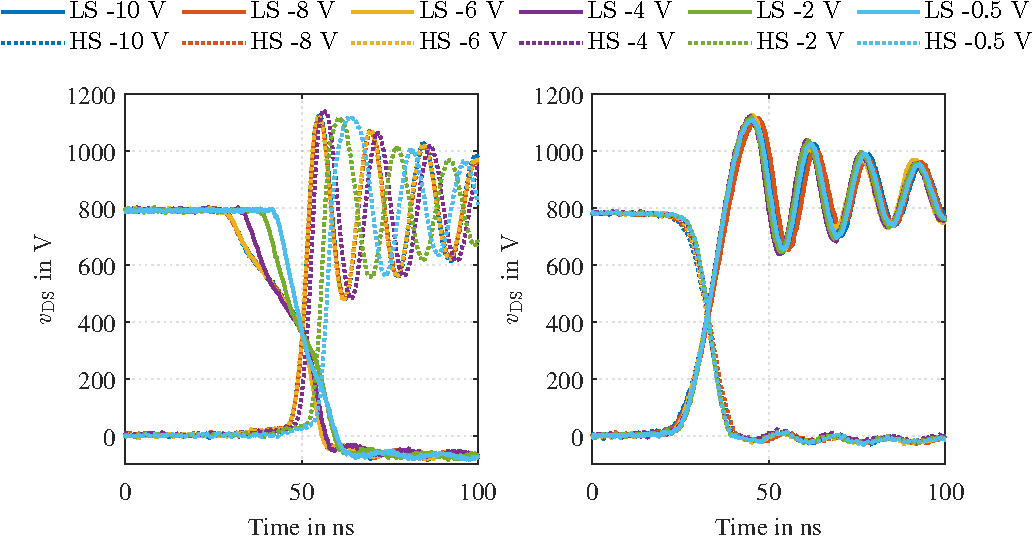
\includegraphics[scale = 1]{figures/7_MeasurementResults/MR_Vee_constOV/MR_Vee_constOV_Voltage_TD.pdf}
		\subcaption{Time-domain voltage measurement results.}
		\label{fig:MR_Vee_constOV_Sweep_Voltage_TD}
	\end{subfigure} 
    
	\vspace{0.5cm}	
	
    \begin{subfigure}[t]{\textwidth}
		\centering
		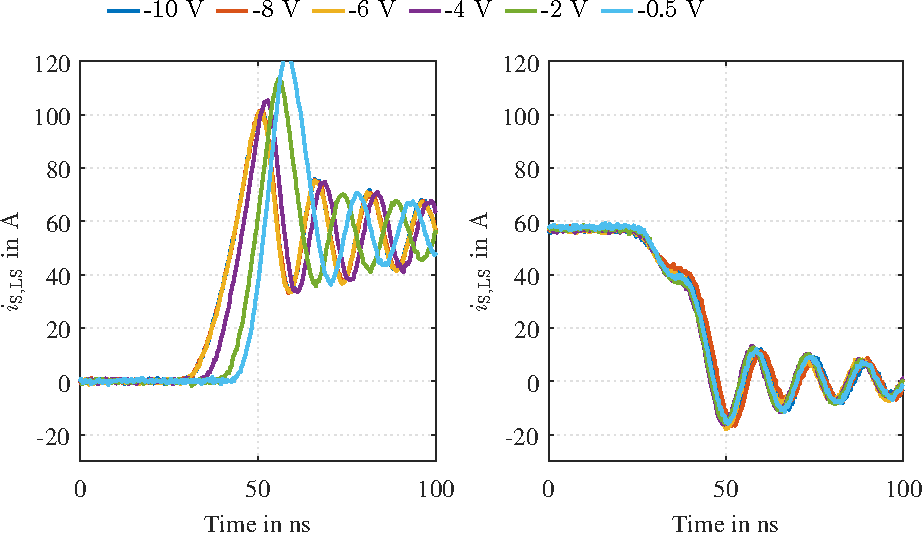
\includegraphics[scale = 1]{figures/7_MeasurementResults/MR_Vee_constOV/MR_Vee_constOV_Current_TD.pdf}
		\subcaption{Time-domain current measurement results.}
		\label{fig:MR_Vee_constOV_Sweep_Current_TD}
	\end{subfigure}
	\caption{Time-domain results of the negative gate-driver bias sweep.}
\end{figure}

\begin{figure}[ht]
	\centering
	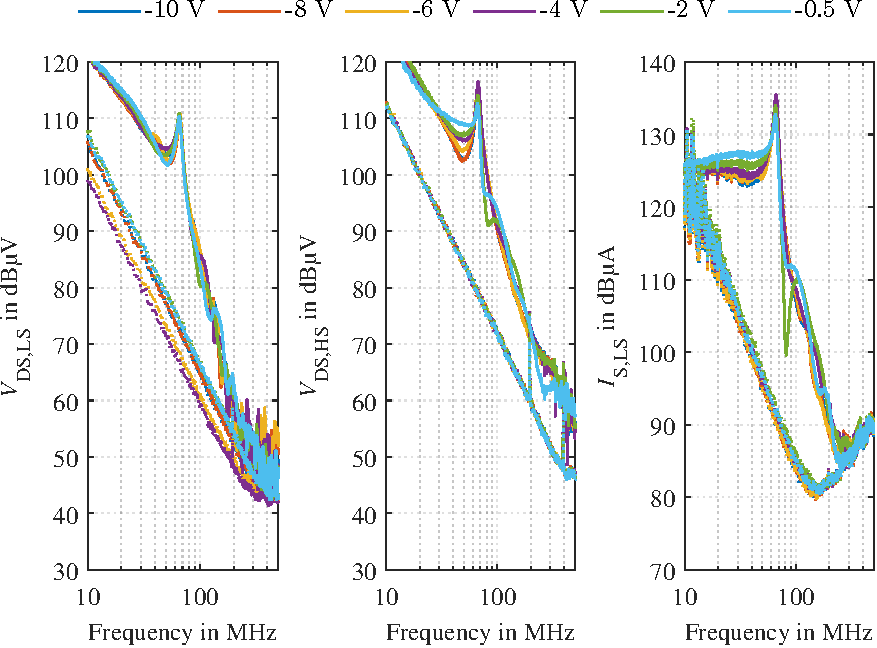
\includegraphics[scale = 1]{figures/7_MeasurementResults/MR_Vee_constOV/MR_Vee_constOV_FD.pdf}
	\caption{Frequency-domain measurement results of the negative gate-driver bias sweep.}\label{fig:MR_Vee_constOV_Sweep_FD}
\end{figure}


\begin{figure}[ht]
	\centering
	\begin{subfigure}[t]{\textwidth}
		\centering
		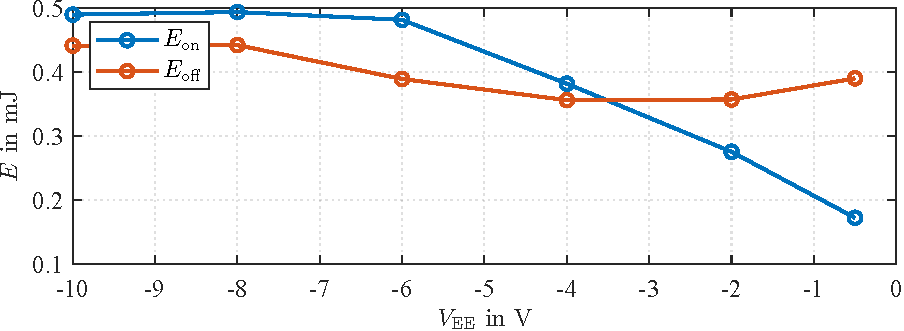
\includegraphics[scale = 1]{figures/7_MeasurementResults/MR_Vee_constOV/MR_Vee_constOV_Losses.pdf}
		\subcaption{Influence of negative gate-driver bias and switching losses on the EM emissions.}
		\label{fig:MR_Vee_constOV_EmissionOverLosses}
	\end{subfigure} 

	\vspace{0.5cm}
	
    \begin{subfigure}[t]{\textwidth}
		\centering
		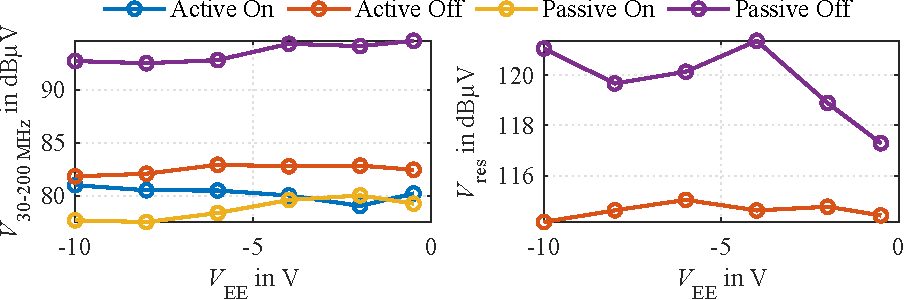
\includegraphics[scale = 1]{figures/7_MeasurementResults/MR_Vee_constOV/MR_Vee_constOV_Emission.pdf}
		\subcaption{EM emissions separated for turn-on and turn-off.}
		\label{fig:MR_Vee_constOV_Emission}
	\end{subfigure}
	\caption{Negative gate-driver-bias-dependent emission and loss analysis for constant overvoltage.}
\end{figure}


\FloatBarrier
\subsection*{Active Chip Area}

\begin{figure}[ht]
	\centering
	\begin{subfigure}[t]{\textwidth}
		\centering
		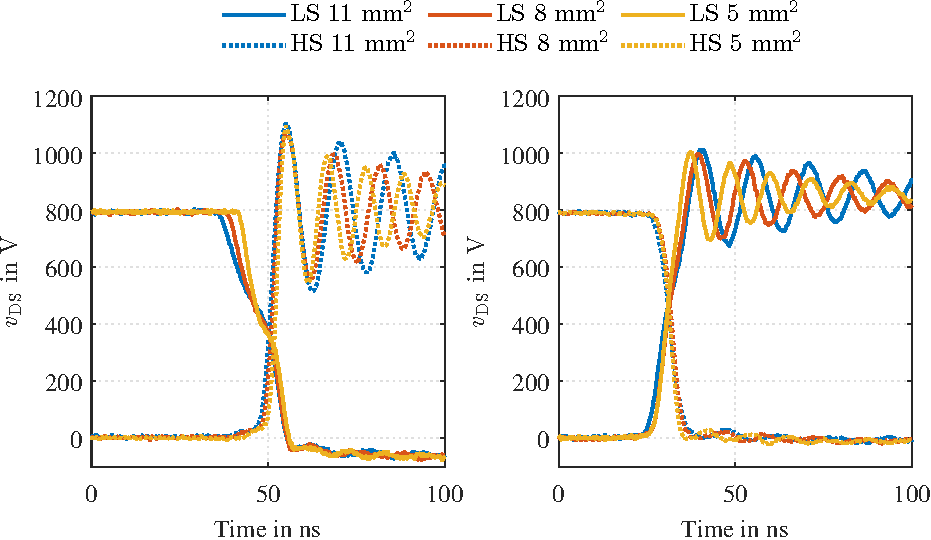
\includegraphics[scale = 1]{figures/7_MeasurementResults/MR_A_constOV/MR_A_constOV_Voltage_TD.pdf}
		\subcaption{Time-domain voltage measurement results.}
		\label{fig:MR_A_constOV_Sweep_Voltage_TD}
	\end{subfigure} 
    
	\vspace{0.5cm}	
	
    \begin{subfigure}[t]{\textwidth}
		\centering
		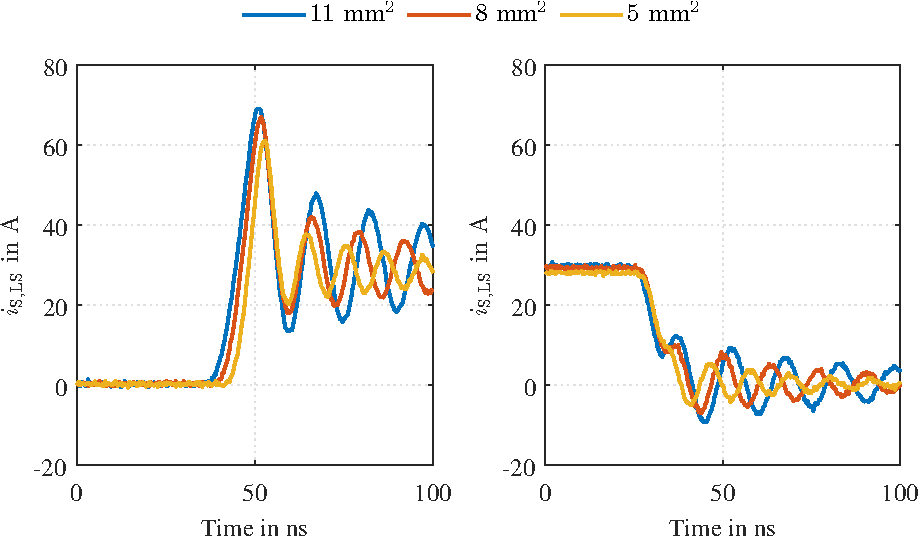
\includegraphics[scale = 1]{figures/7_MeasurementResults/MR_A_constOV/MR_A_constOV_Current_TD.pdf}
		\subcaption{Time-domain current measurement results.}
		\label{fig:MR_A_constOV_Sweep_Current_TD}
	\end{subfigure}
	\caption{Time-domain results of the active-chip-area sweep.}
\end{figure}

\begin{figure}[ht]
	\centering
	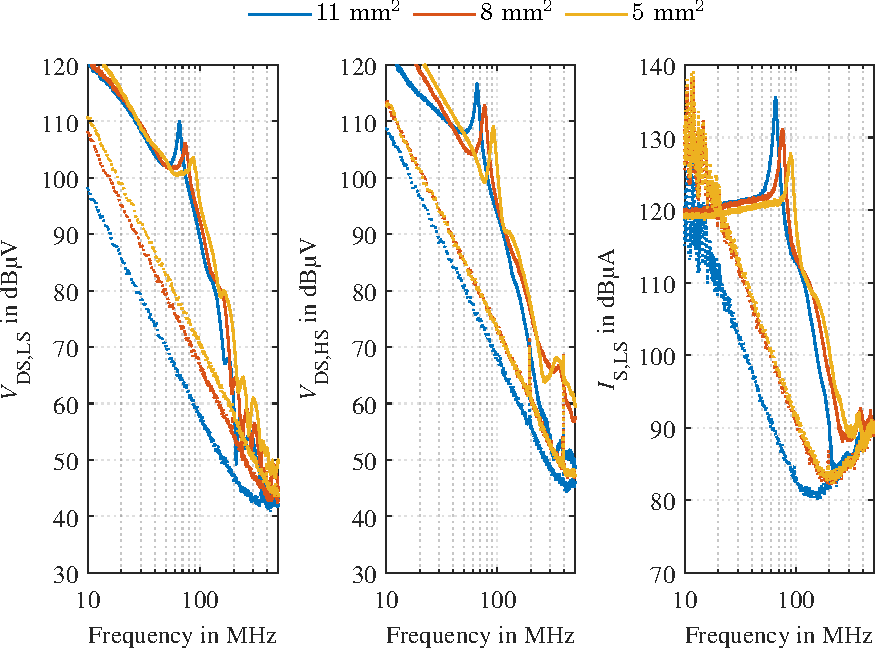
\includegraphics[scale = 1]{figures/7_MeasurementResults/MR_A_constOV/MR_A_constOV_FD.pdf}
	\caption{Frequency-domain measurement results of the active-chip-area sweep.}\label{fig:MR_A_constOV_Sweep_FD}
\end{figure}


\begin{figure}[ht]
	\centering
	\begin{subfigure}[t]{\textwidth}
		\centering
		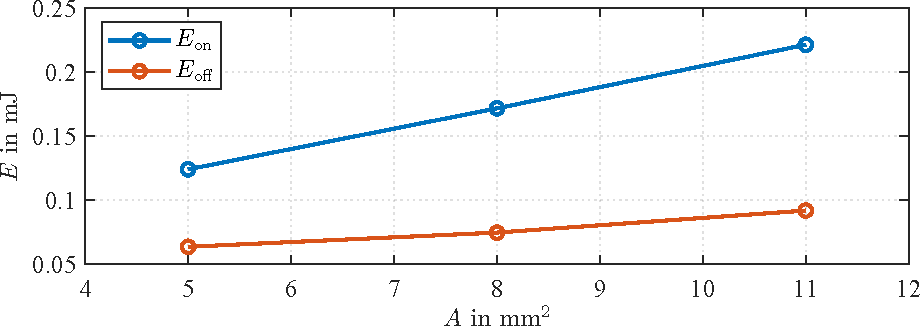
\includegraphics[scale = 1]{figures/7_MeasurementResults/MR_A_constOV/MR_A_constOV_Losses.pdf}
		\subcaption{Influence of active chip area and switching losses on the EM emissions.}
		\label{fig:MR_A_constOV_EmissionOverLosses}
	\end{subfigure} 

	\vspace{0.5cm}
	
    \begin{subfigure}[t]{\textwidth}
		\centering
		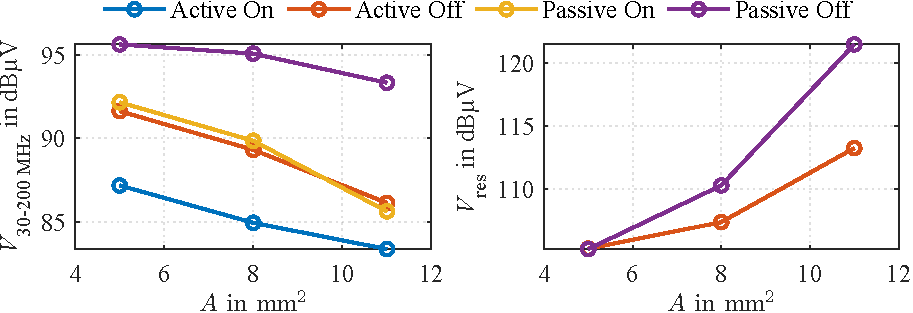
\includegraphics[scale = 1]{figures/7_MeasurementResults/MR_A_constOV/MR_A_constOV_Emission.pdf}
		\subcaption{EM emissions separated for turn-on and turn-off.}
		\label{fig:MR_A_constOV_Emission}
	\end{subfigure}
	\caption{Active-chip-area-dependent emission and loss analysis for constant overvoltage.}
\end{figure}


\FloatBarrier
\subsection*{SiC Technology Generation}


\begin{figure}[ht]
	\centering
	\begin{subfigure}[t]{\textwidth}
		\centering
		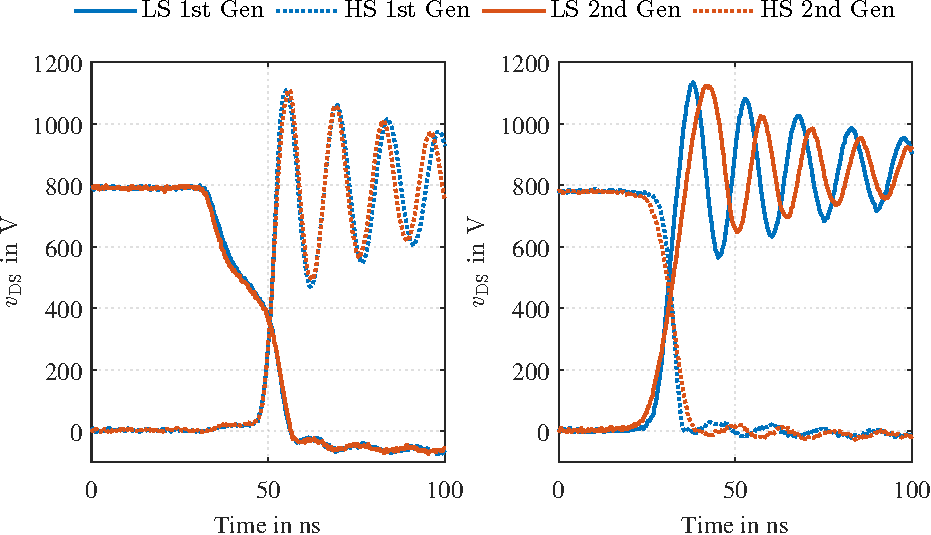
\includegraphics[scale = 1]{figures/7_MeasurementResults/MR_Gen_constOV/MR_Gen_constOV_Voltage_TD.pdf}
		\subcaption{Time-domain voltage measurement results.}
		\label{fig:MR_Gen_constOV_Sweep_Voltage_TD}
	\end{subfigure} 
    
	\vspace{0.5cm}	
	
    \begin{subfigure}[t]{\textwidth}
		\centering
		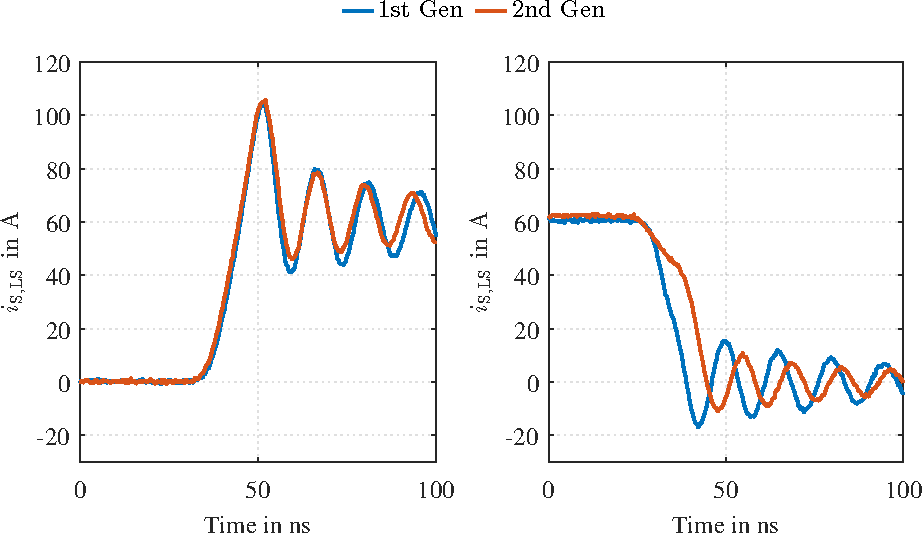
\includegraphics[scale = 1]{figures/7_MeasurementResults/MR_Gen_constOV/MR_Gen_constOV_Current_TD.pdf}
		\subcaption{Time-domain current measurement results.}
		\label{fig:MR_Gen_constOV_Sweep_Current_TD}
	\end{subfigure}
	\caption{Time-domain results of the SiC-technology-generation sweep.}
\end{figure}

\begin{figure}[ht]
	\centering
	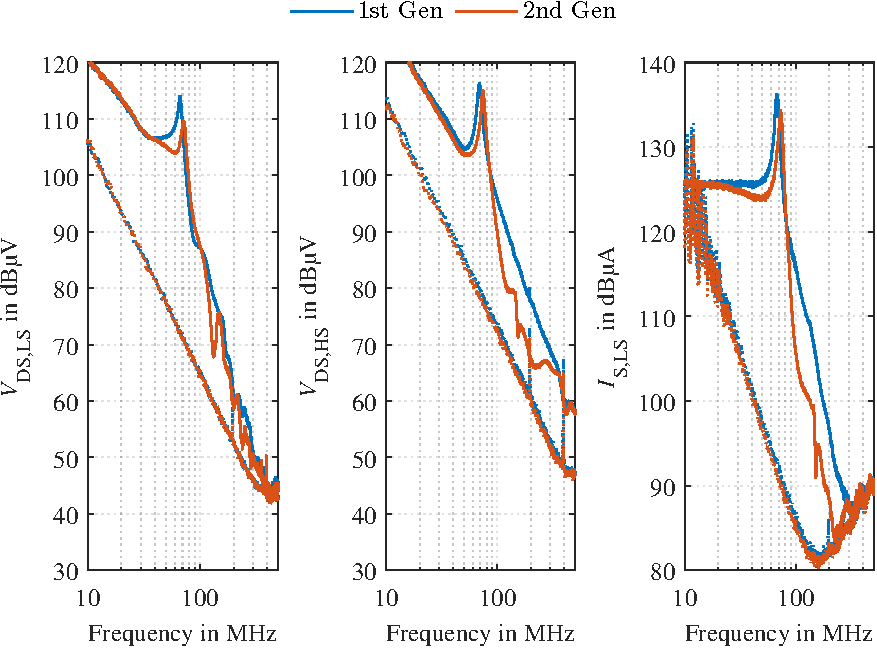
\includegraphics[scale = 1]{figures/7_MeasurementResults/MR_Gen_constOV/MR_Gen_constOV_FD.pdf}
	\caption{Frequency-domain measurement results of the SiC-technology-generation sweep.}\label{fig:MR_Gen_constOV_Sweep_FD}
\end{figure}


\begin{figure}[ht]
	\centering
	\begin{subfigure}[t]{\textwidth}
		\centering
		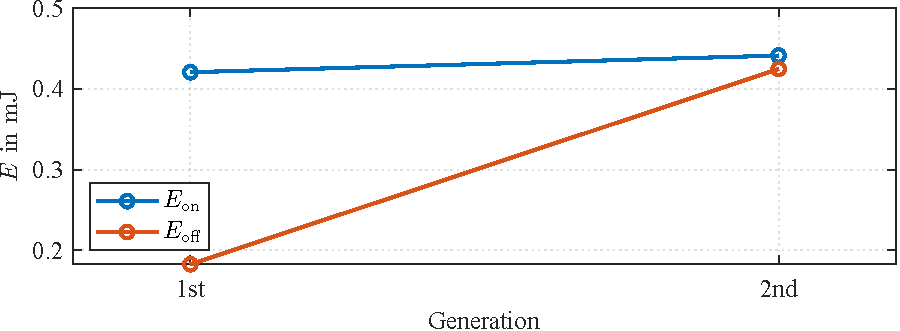
\includegraphics[scale = 1]{figures/7_MeasurementResults/MR_Gen_constOV/MR_Gen_constOV_Losses.pdf}
		\subcaption{Influence of SiC technology generation and switching losses on the EM emissions.}
		\label{fig:MR_Gen_constOV_EmissionOverLosses}
	\end{subfigure} 

	\vspace{0.5cm}
	
    \begin{subfigure}[t]{\textwidth}
		\centering
		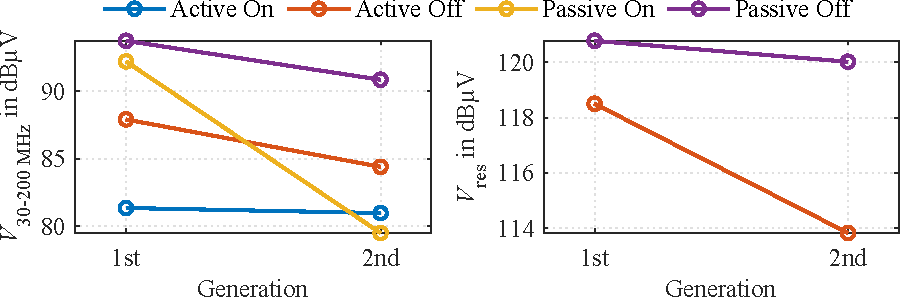
\includegraphics[scale = 1]{figures/7_MeasurementResults/MR_Gen_constOV/MR_Gen_constOV_Emission.pdf}
		\subcaption{EM emissions separated for turn-on and turn-off.}
		\label{fig:MR_Gen_constOV_Emission}
	\end{subfigure}
	\caption{SiC-technology-generation-dependent emission and loss analysis for constant overvoltage.}
\end{figure}


\FloatBarrier
\subsection*{Junction Temperature}

\begin{figure}[ht]
	\centering
	\begin{subfigure}[t]{\textwidth}
		\centering
		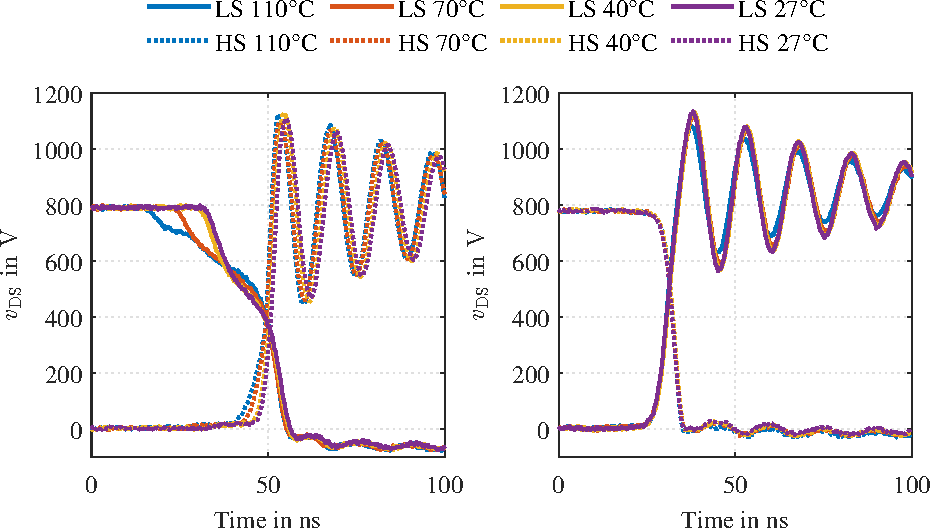
\includegraphics[scale = 1]{figures/7_MeasurementResults/MR_T_constOV/MR_T_constOV_Voltage_TD.pdf}
		\subcaption{Time-domain voltage measurement results.}
		\label{fig:MR_T_constOV_Sweep_Voltage_TD}
	\end{subfigure} 
    
	\vspace{0.5cm}	
	
    \begin{subfigure}[t]{\textwidth}
		\centering
		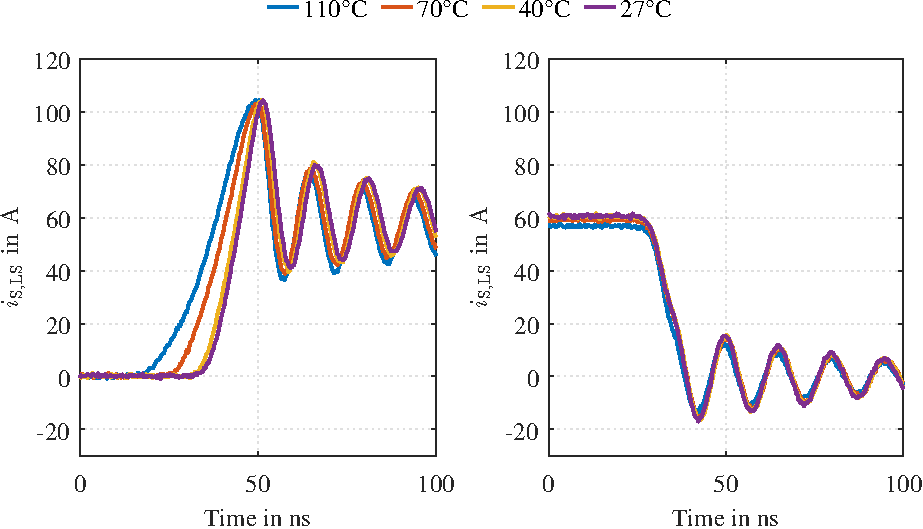
\includegraphics[scale = 1]{figures/7_MeasurementResults/MR_T_constOV/MR_T_constOV_Current_TD.pdf}
		\subcaption{Time-domain current measurement results.}
		\label{fig:MR_T_constOV_Sweep_Current_TD}
	\end{subfigure}
	\caption{Time-domain results of the case-temperature sweep.}
\end{figure}

\begin{figure}[ht]
	\centering
	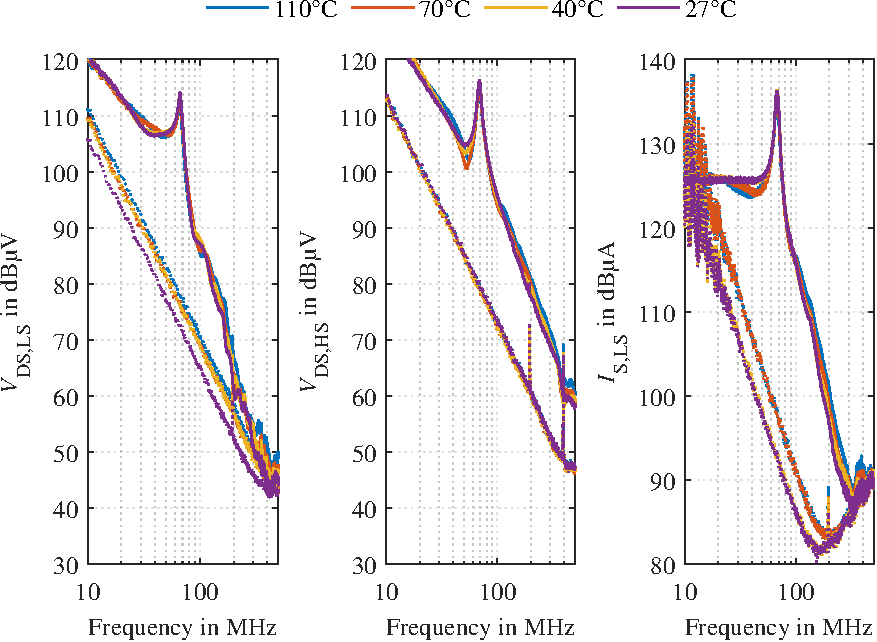
\includegraphics[scale = 1]{figures/7_MeasurementResults/MR_T_constOV/MR_T_constOV_FD.pdf}
	\caption{Frequency-domain measurement results of the case-temperature sweep.}\label{fig:MR_T_constOV_Sweep_FD}
\end{figure}


\begin{figure}[ht]
	\centering
	\begin{subfigure}[t]{\textwidth}
		\centering
		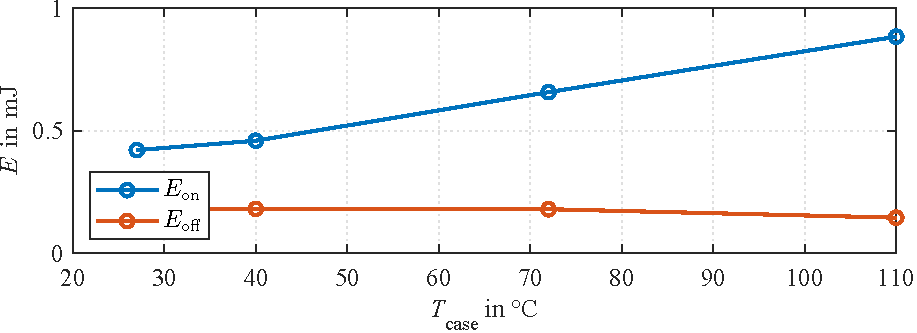
\includegraphics[scale = 1]{figures/7_MeasurementResults/MR_T_constOV/MR_T_constOV_Losses.pdf}
		\subcaption{Influence of junction temperature and switching losses on the EM emissions.}
		\label{fig:MR_T_constOV_EmissionOverLosses}
	\end{subfigure} 

	\vspace{0.5cm}
	
    \begin{subfigure}[t]{\textwidth}
		\centering
		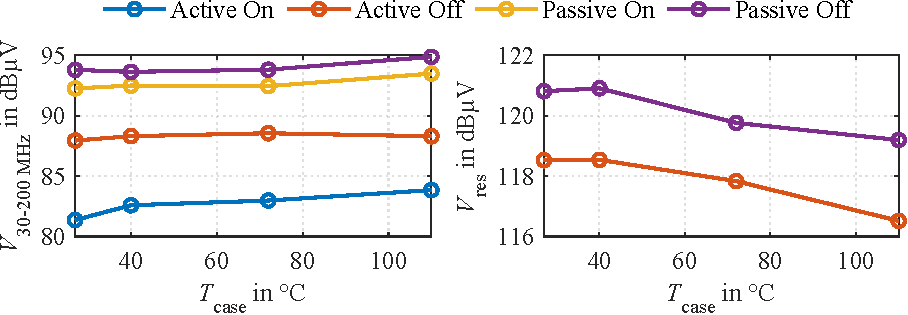
\includegraphics[scale = 1]{figures/7_MeasurementResults/MR_T_constOV/MR_T_constOV_Emission.pdf}
		\subcaption{EM emissions separated for turn-on and turn-off.}
		\label{fig:MR_T_constOV_Emission}
	\end{subfigure}
	\caption{Temperature-dependent emission and loss analysis for constant overvoltage.}
\end{figure}


\FloatBarrier
\subsection*{Commutation-Loop Inductance}


\begin{figure}[ht]
	\centering
	\begin{subfigure}[t]{\textwidth}
		\centering
		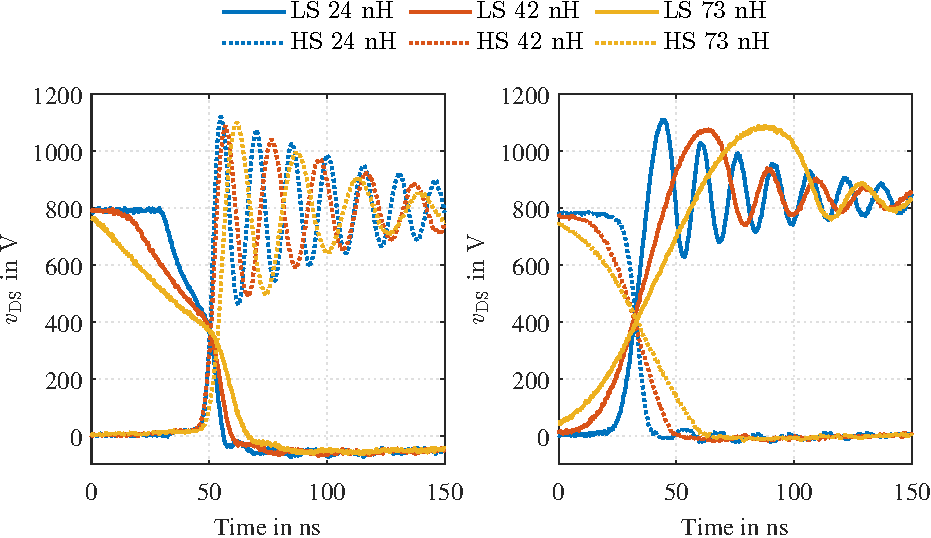
\includegraphics[scale = 1]{figures/7_MeasurementResults/MR_L_constOV/MR_L_constOV_Voltage_TD.pdf}
		\subcaption{Time-domain voltage measurement results.}
		\label{fig:MR_L_constOV_Sweep_Voltage_TD}
	\end{subfigure} 
    
	\vspace{0.5cm}	
	
    \begin{subfigure}[t]{\textwidth}
		\centering
		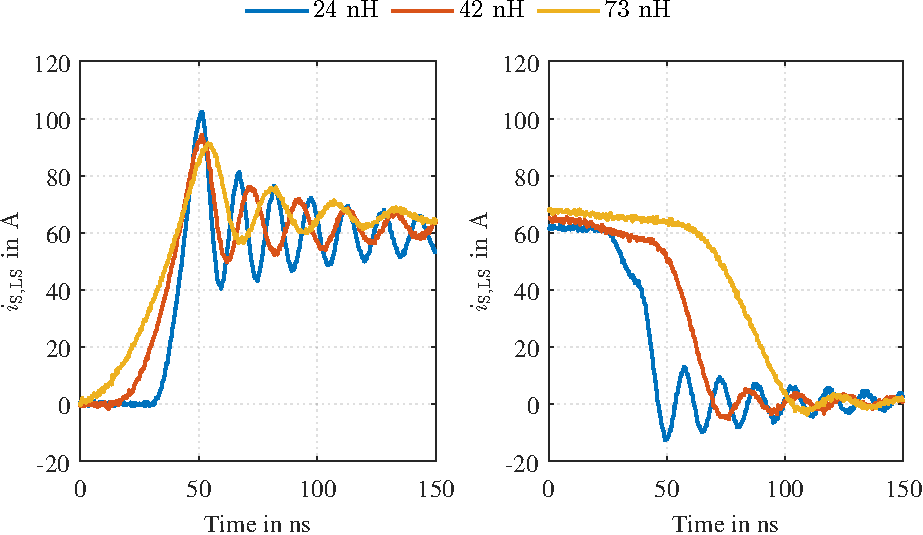
\includegraphics[scale = 1]{figures/7_MeasurementResults/MR_L_constOV/MR_L_constOV_Current_TD.pdf}
		\subcaption{Time-domain current measurement results.}
		\label{fig:MR_L_constOV_Sweep_Current_TD}
	\end{subfigure}
	\caption{Time-domain results of the commutation-loop-inductance sweep.}
\end{figure}

\begin{figure}[ht]
	\centering
	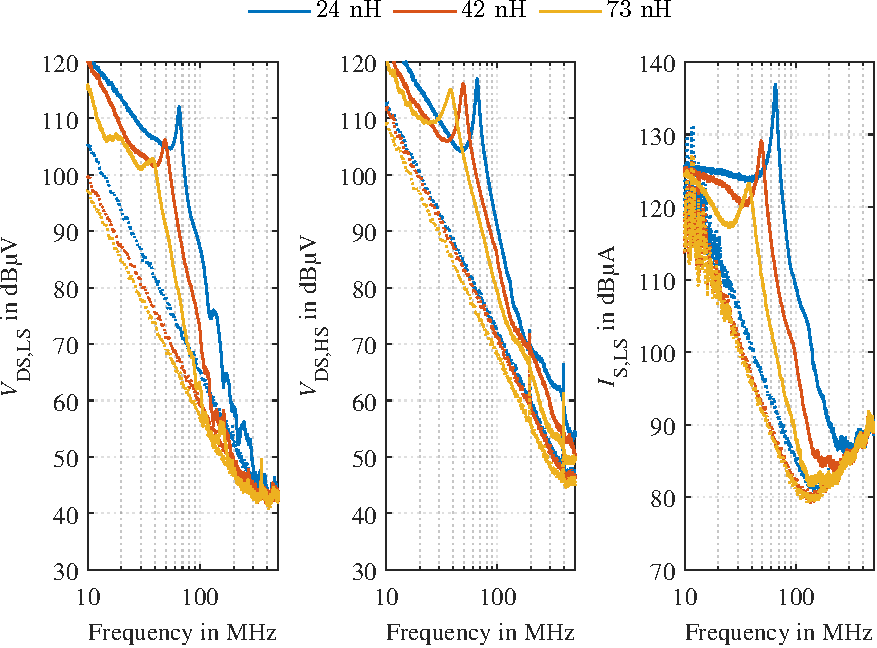
\includegraphics[scale = 1]{figures/7_MeasurementResults/MR_L_constOV/MR_L_constOV_FD.pdf}
	\caption{Frequency-domain measurement results of the commutation-loop-inductance sweep.}\label{fig:MR_L_constOV_Sweep_FD}
\end{figure}


\begin{figure}[ht]
	\centering
	\begin{subfigure}[t]{\textwidth}
		\centering
		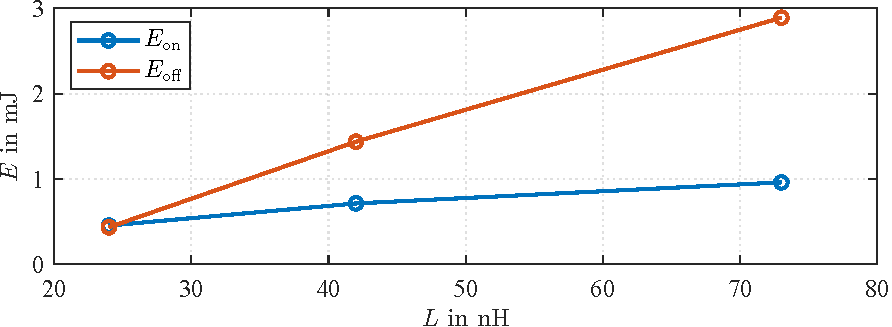
\includegraphics[scale = 1]{figures/7_MeasurementResults/MR_L_constOV/MR_L_constOV_Losses.pdf}
		\subcaption{Influence of commutation-loop inductance and switching losses on the EM emissions.}
		\label{fig:MR_L_constOV_EmissionOverLosses}
	\end{subfigure} 

	\vspace{0.5cm}
	
    \begin{subfigure}[t]{\textwidth}
		\centering
		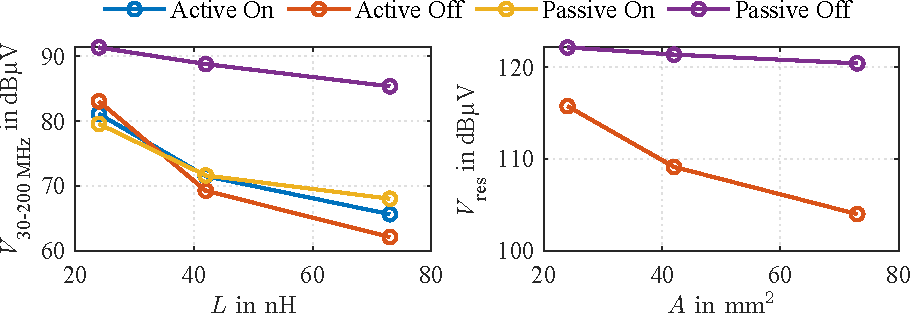
\includegraphics[scale = 1]{figures/7_MeasurementResults/MR_L_constOV/MR_L_constOV_Emission.pdf}
		\subcaption{EM emissions separated for turn-on and turn-off.}
		\label{fig:MR_L_constOV_Emission}
	\end{subfigure}
	\caption{Commutation-loop-inductance-dependent emission and loss analysis for constant overvoltage.}
\end{figure}


 
\FloatBarrier
\section{Comparison Constraint: Constant Gate Resistance}

\subsection*{Negative Gate-Driver Bias}

\begin{figure}[ht]
	\centering
	\begin{subfigure}[t]{\textwidth}
		\centering
		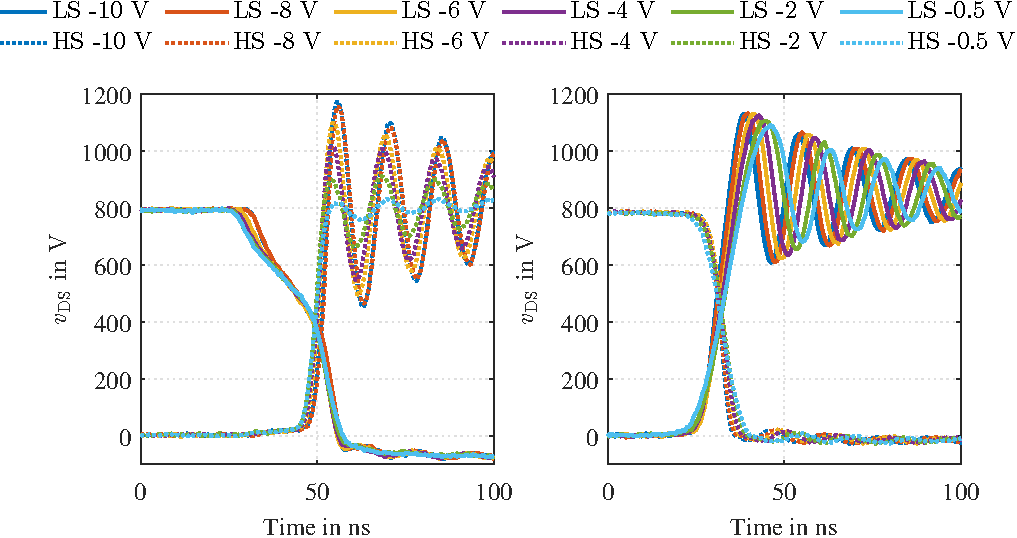
\includegraphics[scale = 1]{figures/7_MeasurementResults/MR_Vee_constRg/MR_Vee_constRg_Voltage_TD.pdf}
		\subcaption{Time-domain voltage measurement results.}
		\label{fig:MR_Vee_constRg_Sweep_Voltage_TD}
	\end{subfigure} 
    
	\vspace{0.5cm}	
	
    \begin{subfigure}[t]{\textwidth}
		\centering
		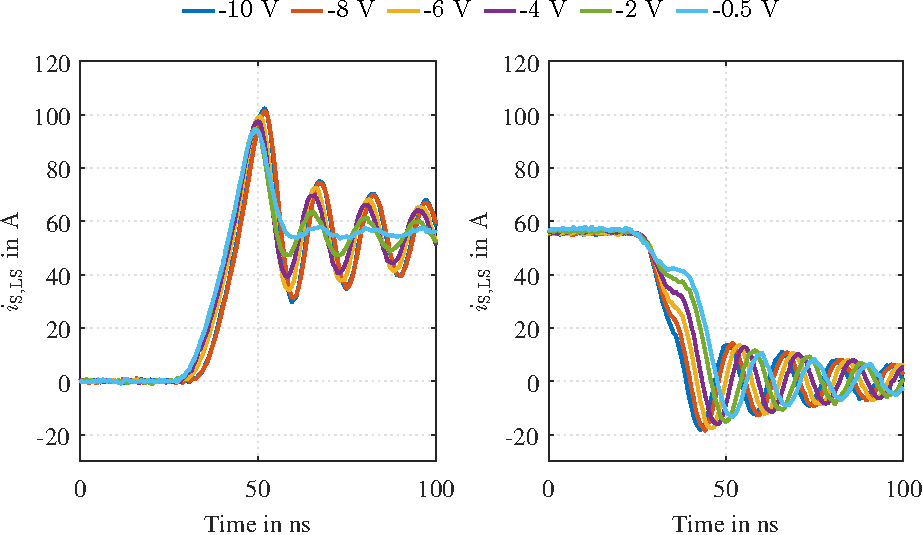
\includegraphics[scale = 1]{figures/7_MeasurementResults/MR_Vee_constRg/MR_Vee_constRg_Current_TD.pdf}
		\subcaption{Time-domain current measurement results.}
		\label{fig:MR_Vee_constRg_Sweep_Current_TD}
	\end{subfigure}
	\caption{Time-domain results of the negative gate-driver bias sweep.}
\end{figure}

\begin{figure}[ht]
	\centering
	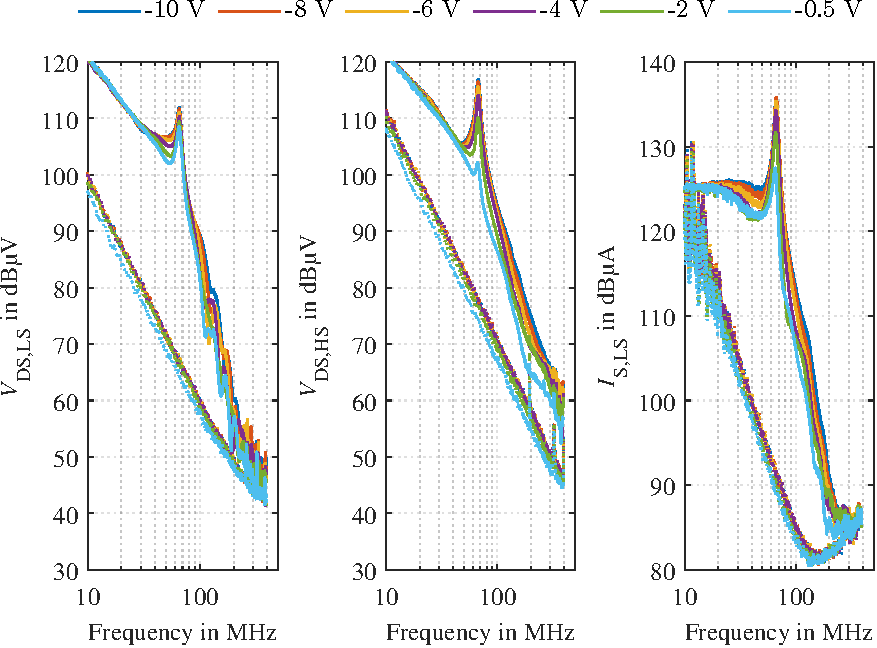
\includegraphics[scale = 1]{figures/7_MeasurementResults/MR_Vee_constRg/MR_Vee_constRg_FD.pdf}
	\caption{Frequency-domain measurement results of the negative gate-driver bias sweep.}\label{fig:MR_Vee_constR_Sweep_FD}
\end{figure}


\begin{figure}[ht]
	\centering
	\begin{subfigure}[t]{\textwidth}
		\centering
		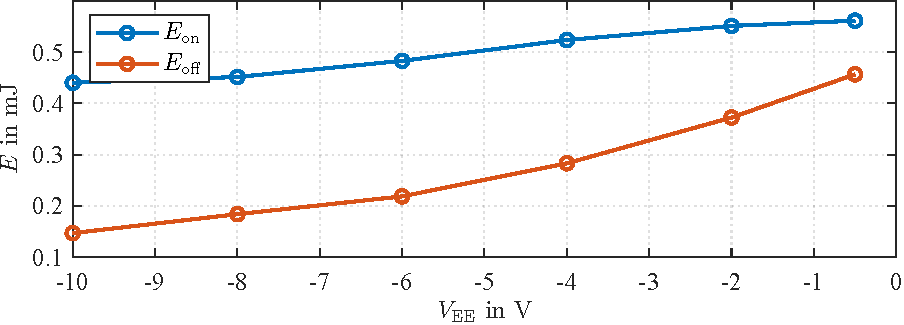
\includegraphics[scale = 1]{figures/7_MeasurementResults/MR_Vee_constRg/MR_Vee_constRg_Losses.pdf}
		\subcaption{Influence of negative gate-driver bias and switching losses on the EM emissions.}
		\label{fig:MR_Vee_constR_EmissionOverLosses}
	\end{subfigure} 

	\vspace{0.5cm}
	
    \begin{subfigure}[t]{\textwidth}
		\centering
		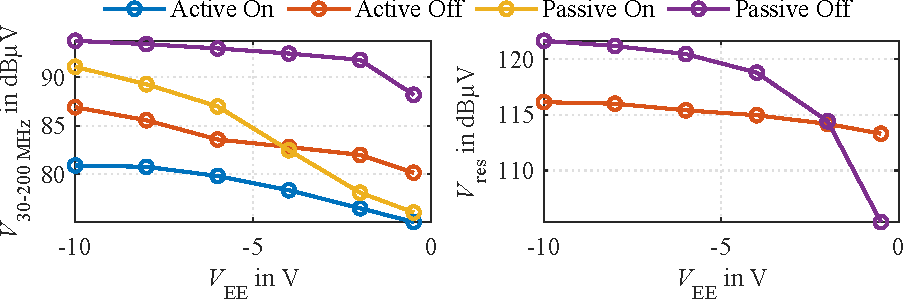
\includegraphics[scale = 1]{figures/7_MeasurementResults/MR_Vee_constRg/MR_Vee_constRg_Emission.pdf}
		\subcaption{EM emissions separated for turn-on and turn-off.}
		\label{fig:MR_Vee_constRg_Emission}
	\end{subfigure}
	\caption{Negative gate-driver-bias-dependent emission and loss analysis for constant gate resistance.}
\end{figure}


\FloatBarrier
\subsection*{Active Chip Area}

\begin{figure}[ht]
	\centering
	\begin{subfigure}[t]{\textwidth}
		\centering
		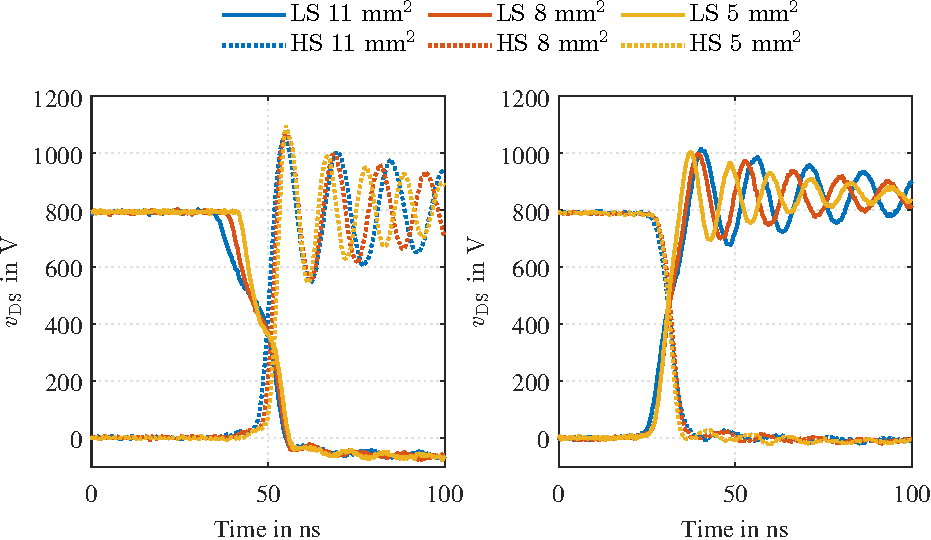
\includegraphics[scale = 1]{figures/7_MeasurementResults/MR_A_constR/MR_A_constR_Voltage_TD.pdf}
		\subcaption{Time-domain voltage measurement results.}
		\label{fig:MR_A_constR_Sweep_Voltage_TD}
	\end{subfigure} 
    
	\vspace{0.5cm}	
	
    \begin{subfigure}[t]{\textwidth}
		\centering
		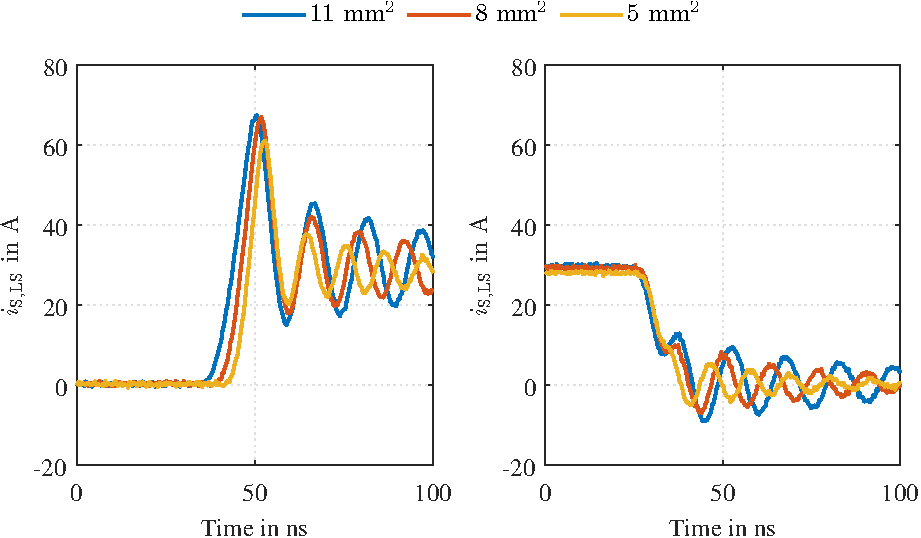
\includegraphics[scale = 1]{figures/7_MeasurementResults/MR_A_constR/MR_A_constR_Current_TD.pdf}
		\subcaption{Time-domain current measurement results.}
		\label{fig:MR_A_constR_Sweep_Current_TD}
	\end{subfigure}
	\caption{Time-domain results of the active-chip-area sweep.}
\end{figure}

\begin{figure}[ht]
	\centering
	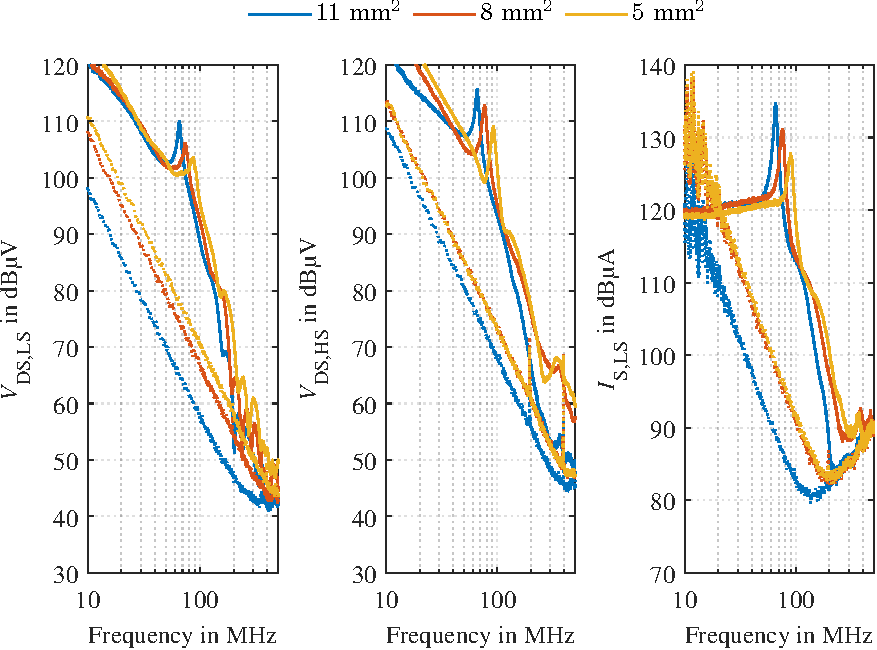
\includegraphics[scale = 1]{figures/7_MeasurementResults/MR_A_constR/MR_A_constR_FD.pdf}
	\caption{Frequency-domain measurement results of the active-chip-area sweep.}\label{fig:MR_A_constR_Sweep_FD}
\end{figure}


\begin{figure}[ht]
	\centering
	\begin{subfigure}[t]{\textwidth}
		\centering
		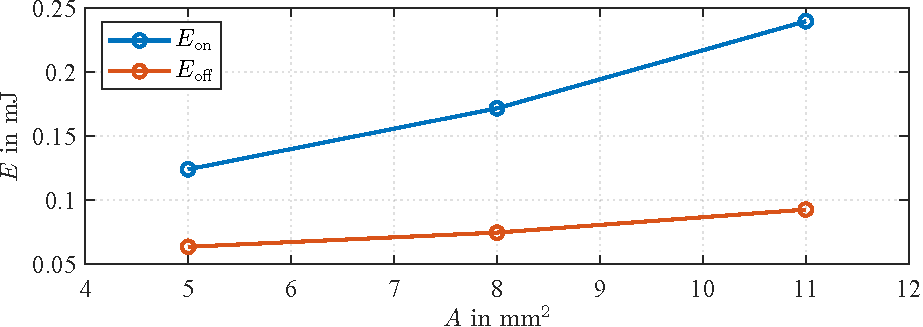
\includegraphics[scale = 1]{figures/7_MeasurementResults/MR_A_constR/MR_A_constR_Losses.pdf}
		\subcaption{Influence of active chip area and switching losses on the EM emissions.}
		\label{fig:MR_A_constR_EmissionOverLosses}
	\end{subfigure} 

	\vspace{0.5cm}
	
    \begin{subfigure}[t]{\textwidth}
		\centering
		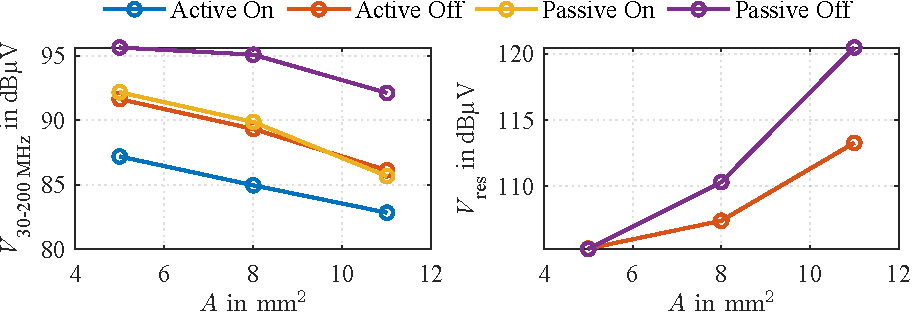
\includegraphics[scale = 1]{figures/7_MeasurementResults/MR_A_constR/MR_A_constR_Emission.pdf}
		\subcaption{EM emissions separated for turn-on and turn-off.}
		\label{fig:MR_A_constR_Emission}
	\end{subfigure}
	\caption{Active-chip-area-dependent emission and loss analysis for constant gate resistance.}
\end{figure}


\FloatBarrier
\subsection*{SiC Technology Generation}


\begin{figure}[ht]
	\centering
	\begin{subfigure}[t]{\textwidth}
		\centering
		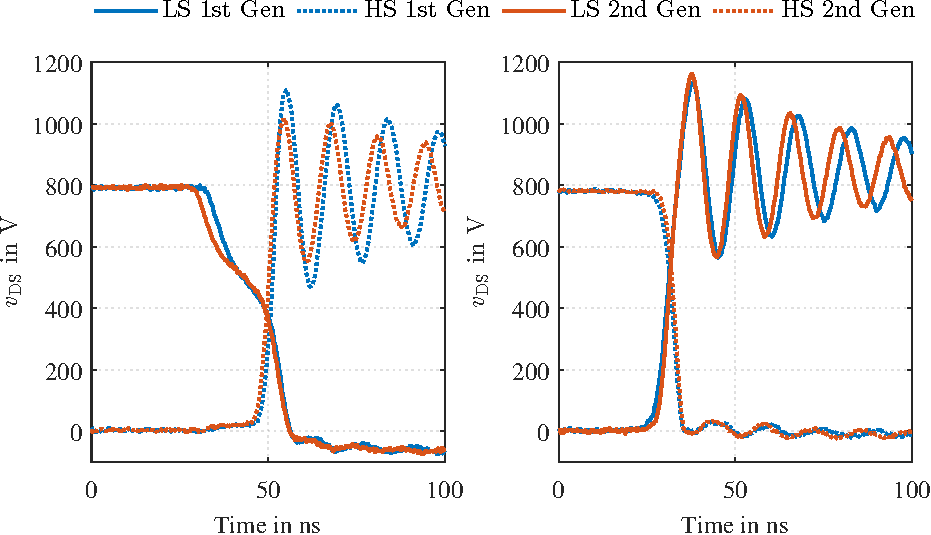
\includegraphics[scale = 1]{figures/7_MeasurementResults/MR_Gen_constR/MR_Gen_constR_Voltage_TD.pdf}
		\subcaption{Time-domain voltage measurement results.}
		\label{fig:MR_Gen_constR_Sweep_Voltage_TD}
	\end{subfigure} 
    
	\vspace{0.5cm}	
	
    \begin{subfigure}[t]{\textwidth}
		\centering
		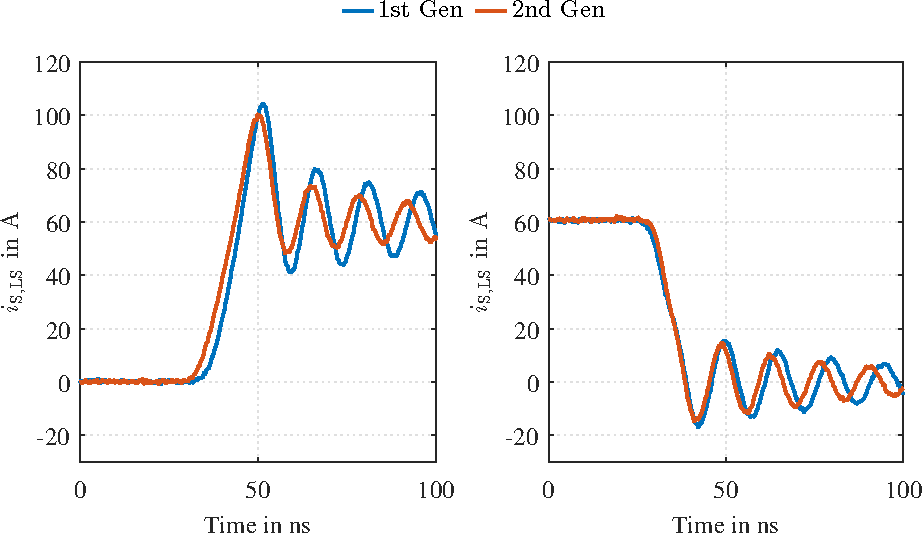
\includegraphics[scale = 1]{figures/7_MeasurementResults/MR_Gen_constR/MR_Gen_constR_Current_TD.pdf}
		\subcaption{Time-domain current measurement results.}
		\label{fig:MR_Gen_constR_Sweep_Current_TD}
	\end{subfigure}
	\caption{Time-domain results of the SiC-technology-generation sweep.}
\end{figure}

\begin{figure}[ht]
	\centering
	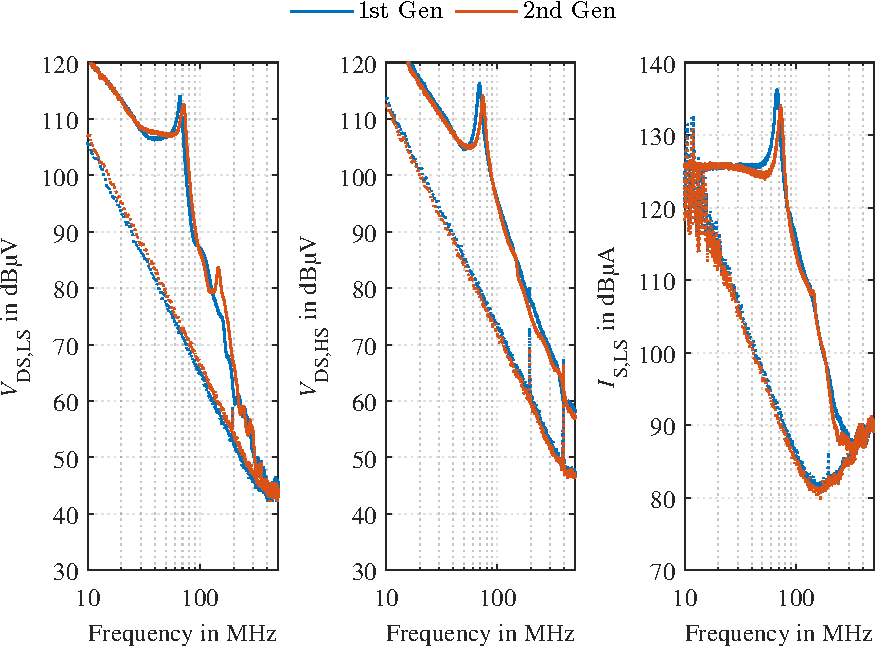
\includegraphics[scale = 1]{figures/7_MeasurementResults/MR_Gen_constR/MR_Gen_constR_FD.pdf}
	\caption{Frequency-domain measurement results of the SiC-technology-generation sweep.}\label{fig:MR_Gen_constR_Sweep_FD}
\end{figure}


\begin{figure}[ht]
	\centering
	\begin{subfigure}[t]{\textwidth}
		\centering
		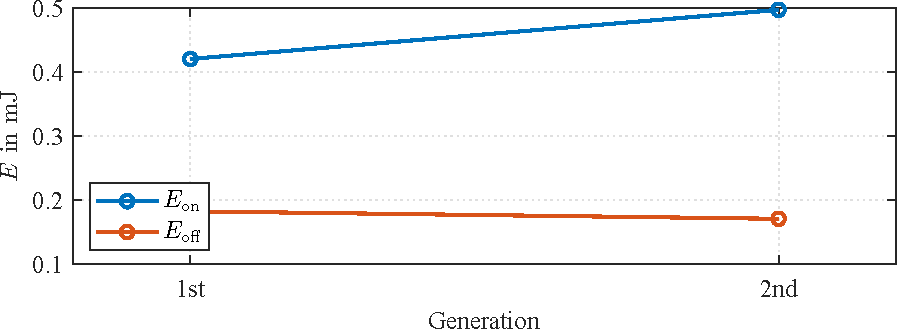
\includegraphics[scale = 1]{figures/7_MeasurementResults/MR_Gen_constR/MR_Gen_constR_Losses.pdf}
		\subcaption{Influence of SiC technology generation and switching losses on the EM emissions.}
		\label{fig:MR_Gen_constR_EmissionOverLosses}
	\end{subfigure} 

	\vspace{0.5cm}
	
    \begin{subfigure}[t]{\textwidth}
		\centering
		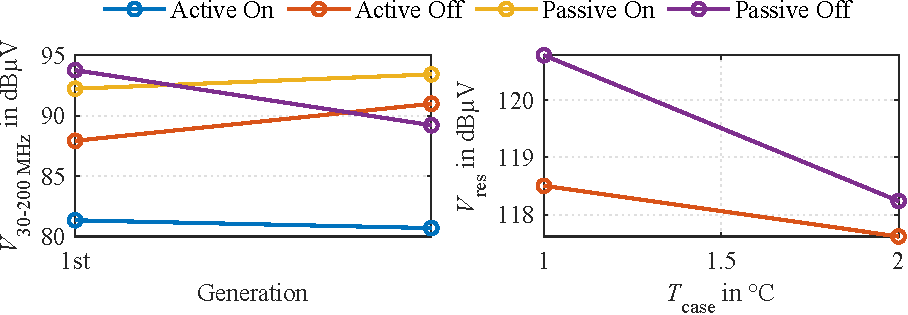
\includegraphics[scale = 1]{figures/7_MeasurementResults/MR_Gen_constR/MR_Gen_constR_Emission.pdf}
		\subcaption{EM emissions separated for turn-on and turn-off.}
		\label{fig:MR_Gen_constR_Emission}
	\end{subfigure}
	\caption{SiC-technology-generation-dependent emission and loss analysis for constant gate resistance.}
\end{figure}


\FloatBarrier
\subsection*{Junction Temperature}

\begin{figure}[ht]
	\centering
	\begin{subfigure}[t]{\textwidth}
		\centering
		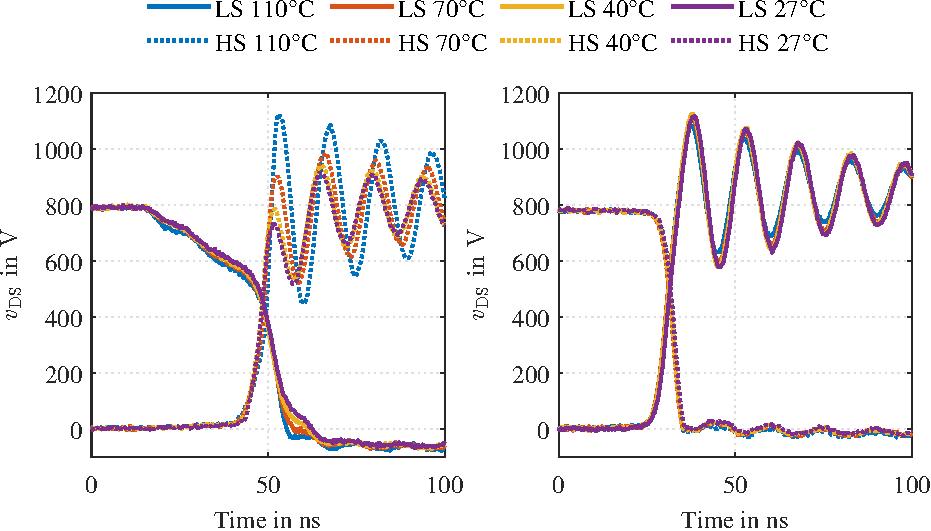
\includegraphics[scale = 1]{figures/7_MeasurementResults/MR_T_constR/MR_T_constR_Voltage_TD.pdf}
		\subcaption{Time-domain voltage measurement results.}
		\label{fig:MR_T_constR_Sweep_Voltage_TD}
	\end{subfigure} 
    
	\vspace{0.5cm}	
	
    \begin{subfigure}[t]{\textwidth}
		\centering
		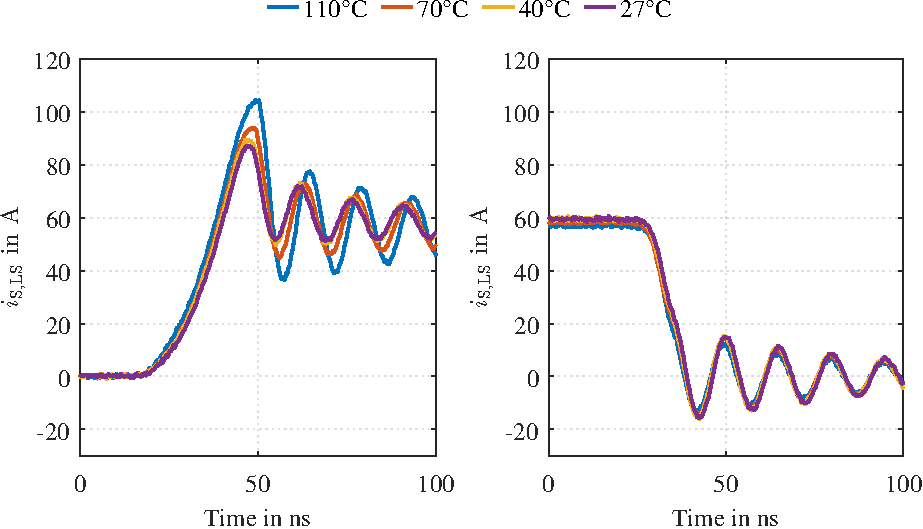
\includegraphics[scale = 1]{figures/7_MeasurementResults/MR_T_constR/MR_T_constR_Current_TD.pdf}
		\subcaption{Time-domain current measurement results.}
		\label{fig:MR_T_constR_Sweep_Current_TD}
	\end{subfigure}
	\caption{Time-domain results of the case-temperature sweep.}
\end{figure}

\begin{figure}[ht]
	\centering
	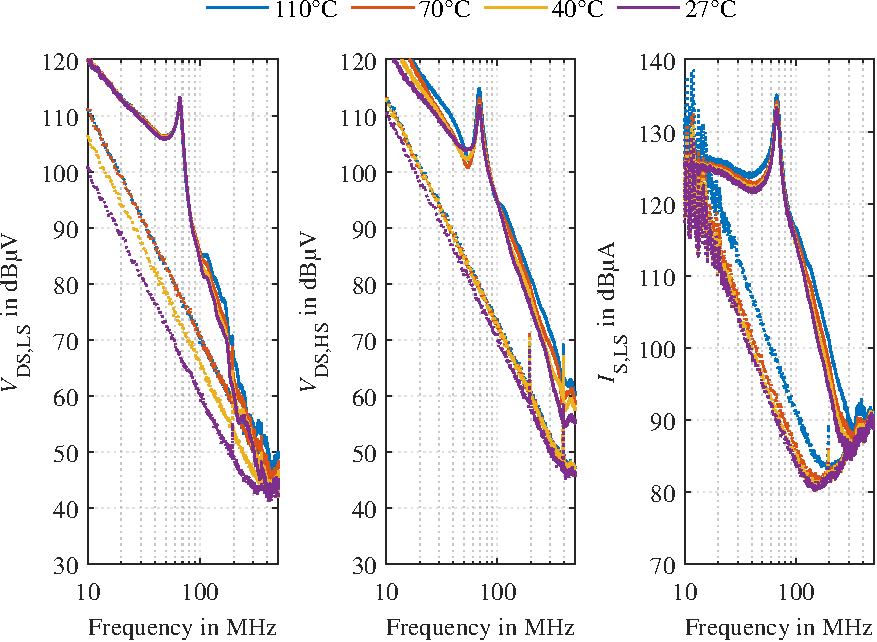
\includegraphics[scale = 1]{figures/7_MeasurementResults/MR_T_constR/MR_T_constR_FD.pdf}
	\caption{Frequency-domain measurement results of the case-temperature sweep.}\label{fig:MR_T_constR_Sweep_FD}
\end{figure}


\begin{figure}[ht]
	\centering
	\begin{subfigure}[t]{\textwidth}
		\centering
		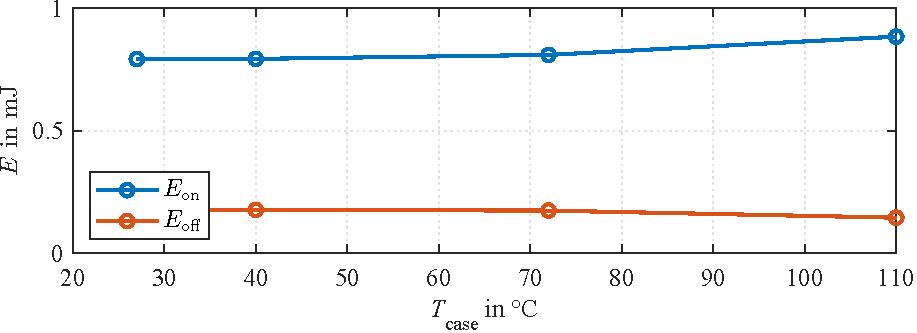
\includegraphics[scale = 1]{figures/7_MeasurementResults/MR_T_constR/MR_T_constR_Losses.pdf}
		\subcaption{Influence of junction temperature and switching losses on the EM emissions.}
		\label{fig:MR_T_constR_EmissionOverLosses}
	\end{subfigure} 

	\vspace{0.5cm}
	
    \begin{subfigure}[t]{\textwidth}
		\centering
		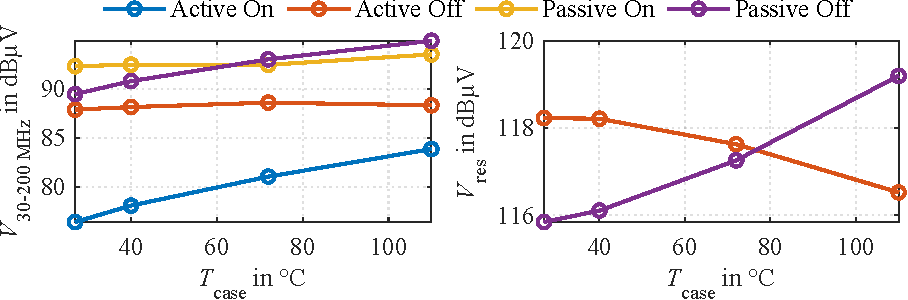
\includegraphics[scale = 1]{figures/7_MeasurementResults/MR_T_constR/MR_T_constR_Emission.pdf}
		\subcaption{EM emissions separated for turn-on and turn-off.}
		\label{fig:MR_T_constR_Emission}
	\end{subfigure}
	\caption{Temperature-dependent emission and loss analysis for constant gate resistance.}
\end{figure}


\FloatBarrier
\subsection*{Commutation-Loop Inductance}


\begin{figure}[ht]
	\centering
	\begin{subfigure}[t]{\textwidth}
		\centering
		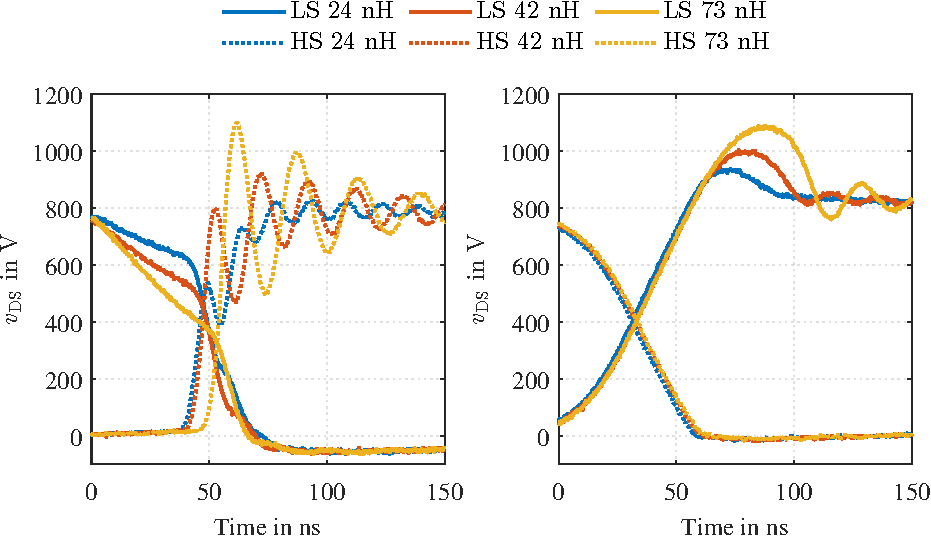
\includegraphics[scale = 1]{figures/7_MeasurementResults/MR_L_constR/MR_L_constR_Voltage_TD.pdf}
		\subcaption{Time-domain voltage measurement results.}
		\label{fig:MR_L_constR_Sweep_Voltage_TD}
	\end{subfigure} 
    
	\vspace{0.5cm}	
	
    \begin{subfigure}[t]{\textwidth}
		\centering
		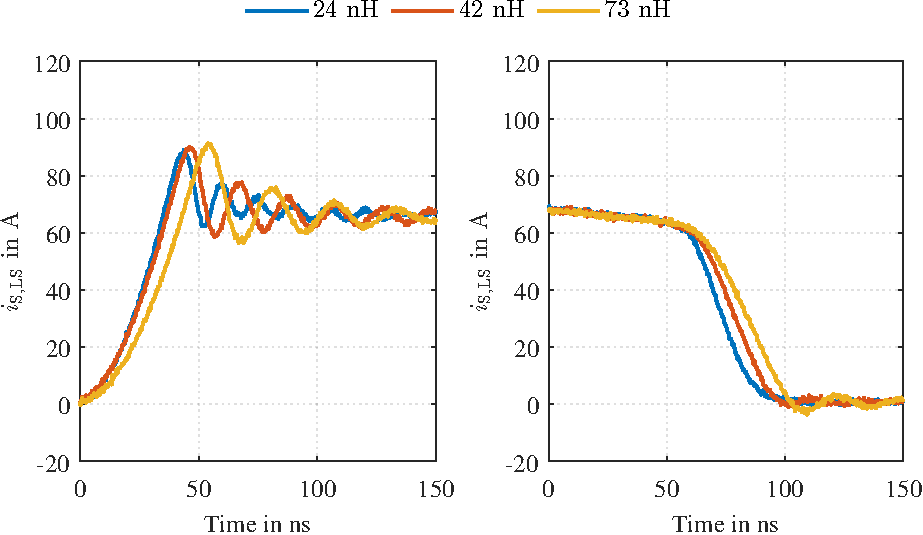
\includegraphics[scale = 1]{figures/7_MeasurementResults/MR_L_constR/MR_L_constR_Current_TD.pdf}
		\subcaption{Time-domain current measurement results.}
		\label{fig:MR_L_constR_Sweep_Current_TD}
	\end{subfigure}
	\caption{Time-domain results of the commutation-loop-inductance sweep.}
\end{figure}

\begin{figure}[ht]
	\centering
	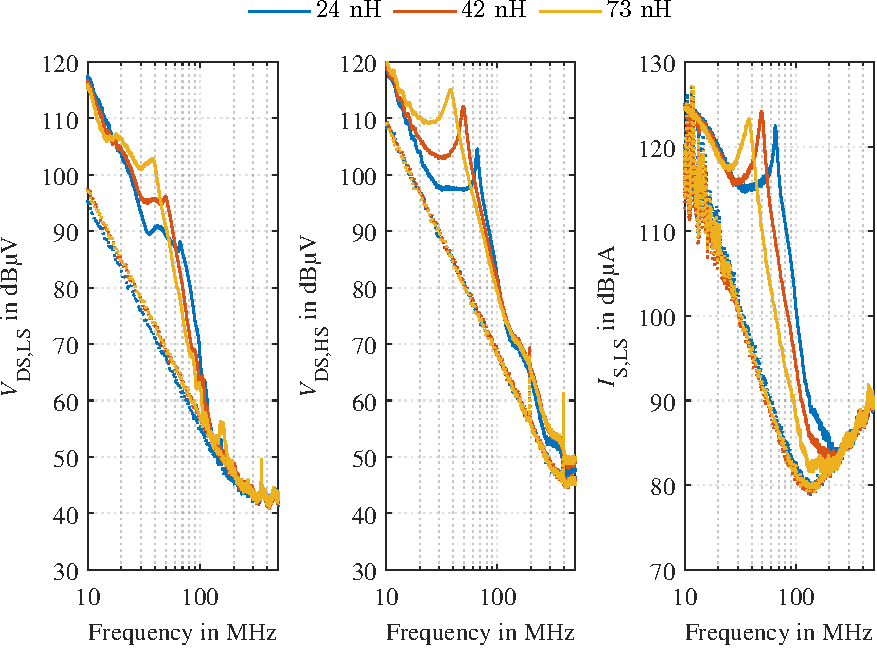
\includegraphics[scale = 1]{figures/7_MeasurementResults/MR_L_constR/MR_L_constR_FD.pdf}
	\caption{Frequency-domain measurement results of the commutation-loop-inductance sweep.}\label{fig:MR_L_constR_Sweep_FD}
\end{figure}


\begin{figure}[ht]
	\centering
	\begin{subfigure}[t]{\textwidth}
		\centering
		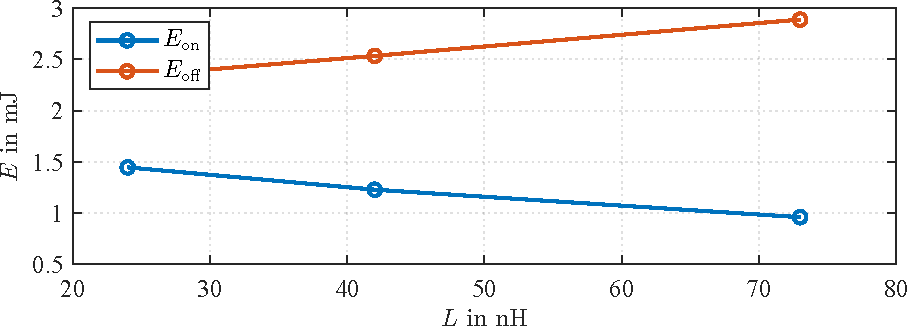
\includegraphics[scale = 1]{figures/7_MeasurementResults/MR_L_constR/MR_L_constR_Losses.pdf}
		\subcaption{Influence of commutation-loop inductance and switching losses on the EM emissions.}
		\label{fig:MR_L_constR_EmissionOverLosses}
	\end{subfigure} 

	\vspace{0.5cm}
	
    \begin{subfigure}[t]{\textwidth}
		\centering
		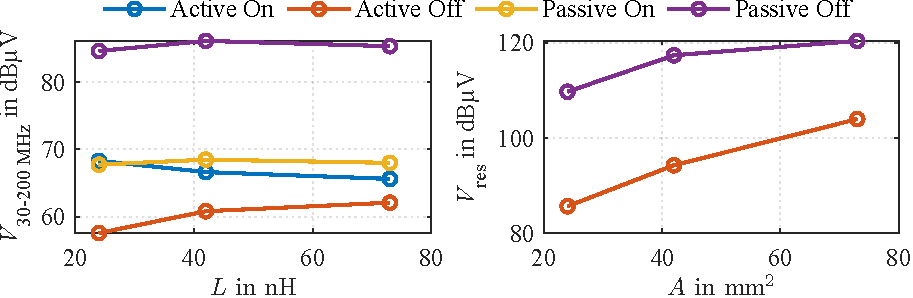
\includegraphics[scale = 1]{figures/7_MeasurementResults/MR_L_constR/MR_L_constR_Emission.pdf}
		\subcaption{EM emissions separated for turn-on and turn-off.}
		\label{fig:MR_L_constR_Emission}
	\end{subfigure}
	\caption{Commutation-loop-inductance-dependent emission and loss analysis for constant gate resistance.}
\end{figure}

